% \iffalse
\let\negmedspace\undefined
\let\negthickspace\undefined
\documentclass[journal,12pt,twocolumn]{IEEEtran}
\usepackage{cite}
\usepackage{amsmath,amssymb,amsfonts,amsthm}
\usepackage{algorithmic}
\usepackage{graphicx}
\usepackage{textcomp}
\usepackage{xcolor}
\usepackage{txfonts}
\usepackage{listings}
\usepackage{enumitem}
\usepackage{mathtools}
\usepackage{gensymb}
\usepackage{comment}
\usepackage[breaklinks=true]{hyperref}
\usepackage{tkz-euclide}
\usepackage{listings}
\usepackage{gvv}
\def\inputGnumericTable{}
\usepackage[latin1]{inputenc}
\usepackage{color}
\usepackage{array}
\usepackage{longtable}
\usepackage{calc}
\usepackage{multirow}
\usepackage{hhline}
\usepackage{ifthen}
\usepackage{lscape}

\newtheorem{theorem}{Theorem}[section]
\newtheorem{problem}{Problem}
\newtheorem{proposition}{Proposition}[section]
\newtheorem{lemma}{Lemma}[section]
\newtheorem{corollary}[theorem]{Corollary}
\newtheorem{example}{Example}[section]
\newtheorem{definition}[problem]{Definition}
\newcommand{\BEQA}{\begin{eqnarray}}
\newcommand{\EEQA}{\end{eqnarray}}
\newcommand{\define}{\stackrel{\triangle}{=}}
\theoremstyle{remark}
\newtheorem{rem}{Remark}
\begin{document}

\bibliographystyle{IEEEtran}
\vspace{3cm}

\title{NCERT Discrete 10.5.2 -15}
\author{EE23BTECH11057 - Shakunaveti Sai Sri Ram Varun$^{}$% &lt;-this % stops a space
}
\maketitle
\newpage
\bigskip

\vspace{2cm}
\textbf{Question: }
For what value of $ n$, are the $ nth$ terms of two A.Ps: 63, 65, 67,\dots and 3, 10, 17,\dots equal?\\
\vspace{0.5cm}
\textbf{Solution}:

\begin{table}[htbp] 
\centering
\begin{tabular}{|c|c|c|}
    \hline
    \textbf{Parameter} & \textbf{Description} & \textbf{Value} \\
    \hline
    $X\brak{s}$ & position in laplace domain & $ X\brak{s}$ \\
    \hline
    $\Theta\brak{s}$ & angle rotated in laplace domain & $ \Theta\brak{s}$ \\
    \hline
    $x\brak{t}$ & position of mass w.r.t time & $x\brak{t}$ \\
    \hline
    $\theta\brak{t}$ & angle rotated by mass w.r.t time &$ \theta\brak{t}$\\
    \hline
    $\alpha\brak{t}$ & angular acceleration of mass w.r.t time & $\alpha\brak{t}$ \\
    \hline
    $k$ & spring constant & $ k$\\
    \hline
    $m$ & mass of the block & $ m$\\
    \hline
    $L$ & length of the mass & $ L$\\
    \hline
    $\omega_o$ & initial angular velocity of mass & $ \omega_o$ \\
    \hline
    $v\brak{0}$ & initial velocity of mass& $ v\brak{0}$ \\
    \hline
    
\end{tabular}






\caption{input values}
\label{tab: Table 1}
\end{table}
\begin{align}
x_i\brak{n} &= x\brak{0}u\brak{n} + dnu\brak{n}\\
from the equation
X\brak{z} &= \frac{x\brak{0}}{1-z^{1}} + \frac{dz^{-1}}{\brak{1-z^{-1}}^{2}} \quad |z|>1\label{eq:5}
\end{align}
\begin{enumerate}
\item
\begin{align}
x_1\brak{n} &= 63u\brak{n} + 2nu\brak{n} \label{eq:3}\\
%To find $ X_1\brak{z}$:
X_1\brak{z} &= \frac{63}{1-z^{1}} + \frac{2z^{-1}}{\brak{1-z^{-1}}^{2}}  \quad |z|>1
\end{align}
\item
\begin{align}
x_2\brak{n} &= 3u\brak{n} + 7nu\brak{n} \label{eq:4}\\ 
%To find $ X_2\brak{z}$ :\\
X_2\brak{z} &= \frac{3}{1-z^{1}} + \frac{7z^{-1}}{\brak{1-z^{-1}}^{2}} \quad |z|>1
\end{align}
\item

given,
\begin{align}
 x_1\brak{n} &= x_2\brak{n}\\
\therefore 63 + 2n &= 7n+3\\
\implies n &=12
\end{align}
\begin{figure}[h!]
    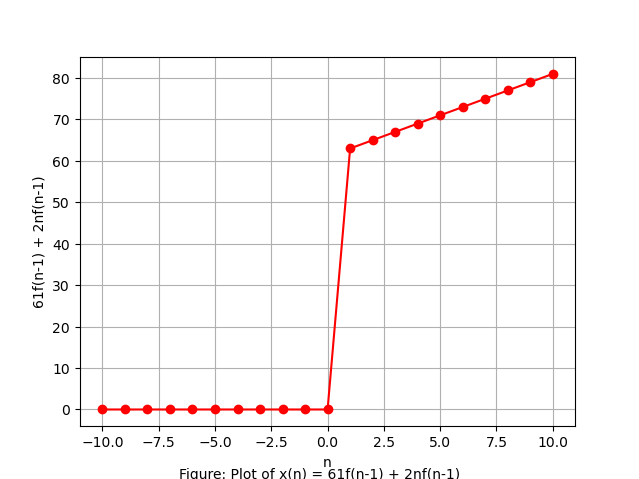
\includegraphics[width = \columnwidth]{Figure_1.png}
    \caption{Graphs of $ x_1\brak{n}$ and $ x_2\brak{n}$ and both are equal at $ n=12$}
    \label{fig: 1}
\end{figure}
\end{enumerate}
\end{document}
